\documentclass[10pt,a4paper,draft]{article}
\usepackage[utf8]{inputenc}
\usepackage{amsmath}
\usepackage{amsfonts}
\usepackage{amssymb}
\usepackage{graphicx}
\usepackage{tikz}

\title{Model for elastic energy of a dissociated dislocation}

\begin{document}
\section{Introduction}
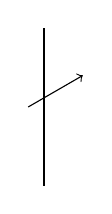
\begin{tikzpicture}
\draw (0,0) -- (0,2);
\draw [->] (-0.2,1) -- ++(30:0.8);
\end{tikzpicture}

The general model for the elastic energy per unit length for a mixed dislocation dissociated into two partials can be given as \cite{bacon78}:
\begin{equation}
E_D(\theta) = E_S(\theta) + E_I(\theta) + E_F(\theta) \label{eqbacon}
\end{equation}
"$E_S$" is the self-energy of the two partials, "$E_I$" is the interaction energy (of the two partials), and "$E_F$" is the fault-energy. "$\theta$" is the angle between the Burgers vector and the unit line vector.\\

A general expression can be given for each energy.
\begin{subequations}
\begin{align}
E_S(\theta) & = \frac{\mu b^2}{4\pi}\left(1-\nu\cos^2\theta\right)\ln\left(\frac{R}{r_0}\right) \label{eq:defEs}\\
E_I(\theta) & = \frac{\mu b^2}{2\pi}\left(\alpha+\frac{\beta}{1-\nu}\right)\ln\left(\frac{R}{\Delta}\right)-\frac{\mu}{2\pi(1-\nu)}\psi \label{eq:defEi}\\
E_F & = \gamma \Delta \label{eq:defEf}
\end{align}
\end{subequations}
$r_0$ and $R$ are the inner and outer cutoff radii, respectively. $\mu$, $b$, and $\nu$ are the shear modulus, the Burgers vector of the dislocation, and the Poisson ratio.\\

Equation \ref{eq:defEi} is the interaction energy between two parallel dislocation segments separated by a vector $\vec{\Delta}$. $\alpha$, $\beta$, and $\psi$ are related to the Burgers vectors and the line direction vectors of the two dislocations. $\Delta$ is the vector pointing from one dislocation segment to the second.

$\gamma$ is the stacking-fault energy

\section{Mixed Shockley dislocation $\beta \pm \pi/6$}

\bibliography{bacon1978.bib}
\bibliographystyle{plain}
\end{document}



